\chapter{Calibration}

\section{From image to camera}
\begin{figure}[h]
\centering
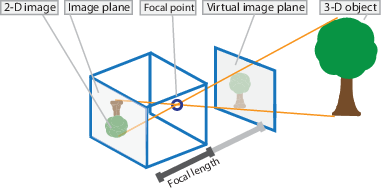
\includegraphics[width=\textwidth]{figures/camera_calibration_focal_point.PNG}
\caption{}
\label{fig:camera_calibration_focal_point}
\end{figure}
When taking an image for the use of detecting an object it is necessary to transform the image frame into the robot frame. First the image has to be transformed from world coordinates into camera coordinates and then to robot coordinates. When going from world to camera the pinhole camera model can be used. A graphical depictions of the model can be seen in \autoref{fig:camera_calibration_focal_point}. The camera is assumed to be box where no light can enter except from a small hole called the focal point. The light that is cast on the back wall is an inverted 2D representation of the 3D world outside of the box. The 2D image depends on the distance from the focal point to the back wall, called the focal length. The transformation is split into two parts; from world coordinate to camera coordinate and from camera coordinates to image coordinates. This is done by finding the intrinsic and extrinsic parameters. The intrinsic paramaters look like this:
\begin{equation}
\begin{bmatrix}
u \\
v \\
w 
\end{bmatrix} 
 =
\begin{bmatrix}
a_x & s & x_0 & 0 \\
0 & a_y & y_0 & 0 \\
0 & 0 & 0 & 0 
\end{bmatrix}  
\begin{bmatrix}
x_s \\
y_s \\
z_s \\
0 
\end{bmatrix}
\end{equation}
where $x_s, y_s, z_s$ are the scene points in the camera coordinate system, $u, v, w$ are the homogenous image coordinates where $w$ is a scaling factor. The parameters are $a_x, a_y$ which are the focal length. $x_0$ and $y_0$ are to translate the image center to be the actual image center since there may be an offset due to fabrication issues.  $s$ is the pixel skew parameter but it is usually set to 0. 

The extrinsic parameters are a translation and rotation that describe where in the world the camera is located and how it is oriented. The parameters can be expressed as:
$ \begin{bmatrix}
R & -RC  \\
0_{3}^{T} & 1 
\end{bmatrix}  $
where $R$ is the rotation and $-RC$ is the is the translation. To get the whole transformation it would look like this:

\begin{equation}
\begin{bmatrix}
u \\
v \\
w 
\end{bmatrix} 
 =
\begin{bmatrix}
a_x & s & x_0 & 0 \\
0 & a_y & y_0 & 0 \\
0 & 0 & 0 & 0 
\end{bmatrix}  
\begin{bmatrix}
R & -RC  \\
0_{3}^{T} & 1 
\end{bmatrix}
\begin{bmatrix}
x_s \\
y_s \\
z_s \\
0 
\end{bmatrix}
\end{equation}

Lastly there can also be some radial distortion in the image cause by the lens which causes lines that are linear in the world coordinate to appear non linear in the image. This correction can be computed by using images with objects with known straight lines. To get all these parameters the Camera Calibration Toolbox for Matlab by Jean-Yves Bouguet can be used.  Here 10 - 20 images are taken of a checkerboard pattern,\autoref{fig:checkerbord_pattern}, where the size of the squares is known and from this, it is possible to estimate the intrinsic and extrinsic parameters and distortion. 

\begin{figure}[h]
\centering
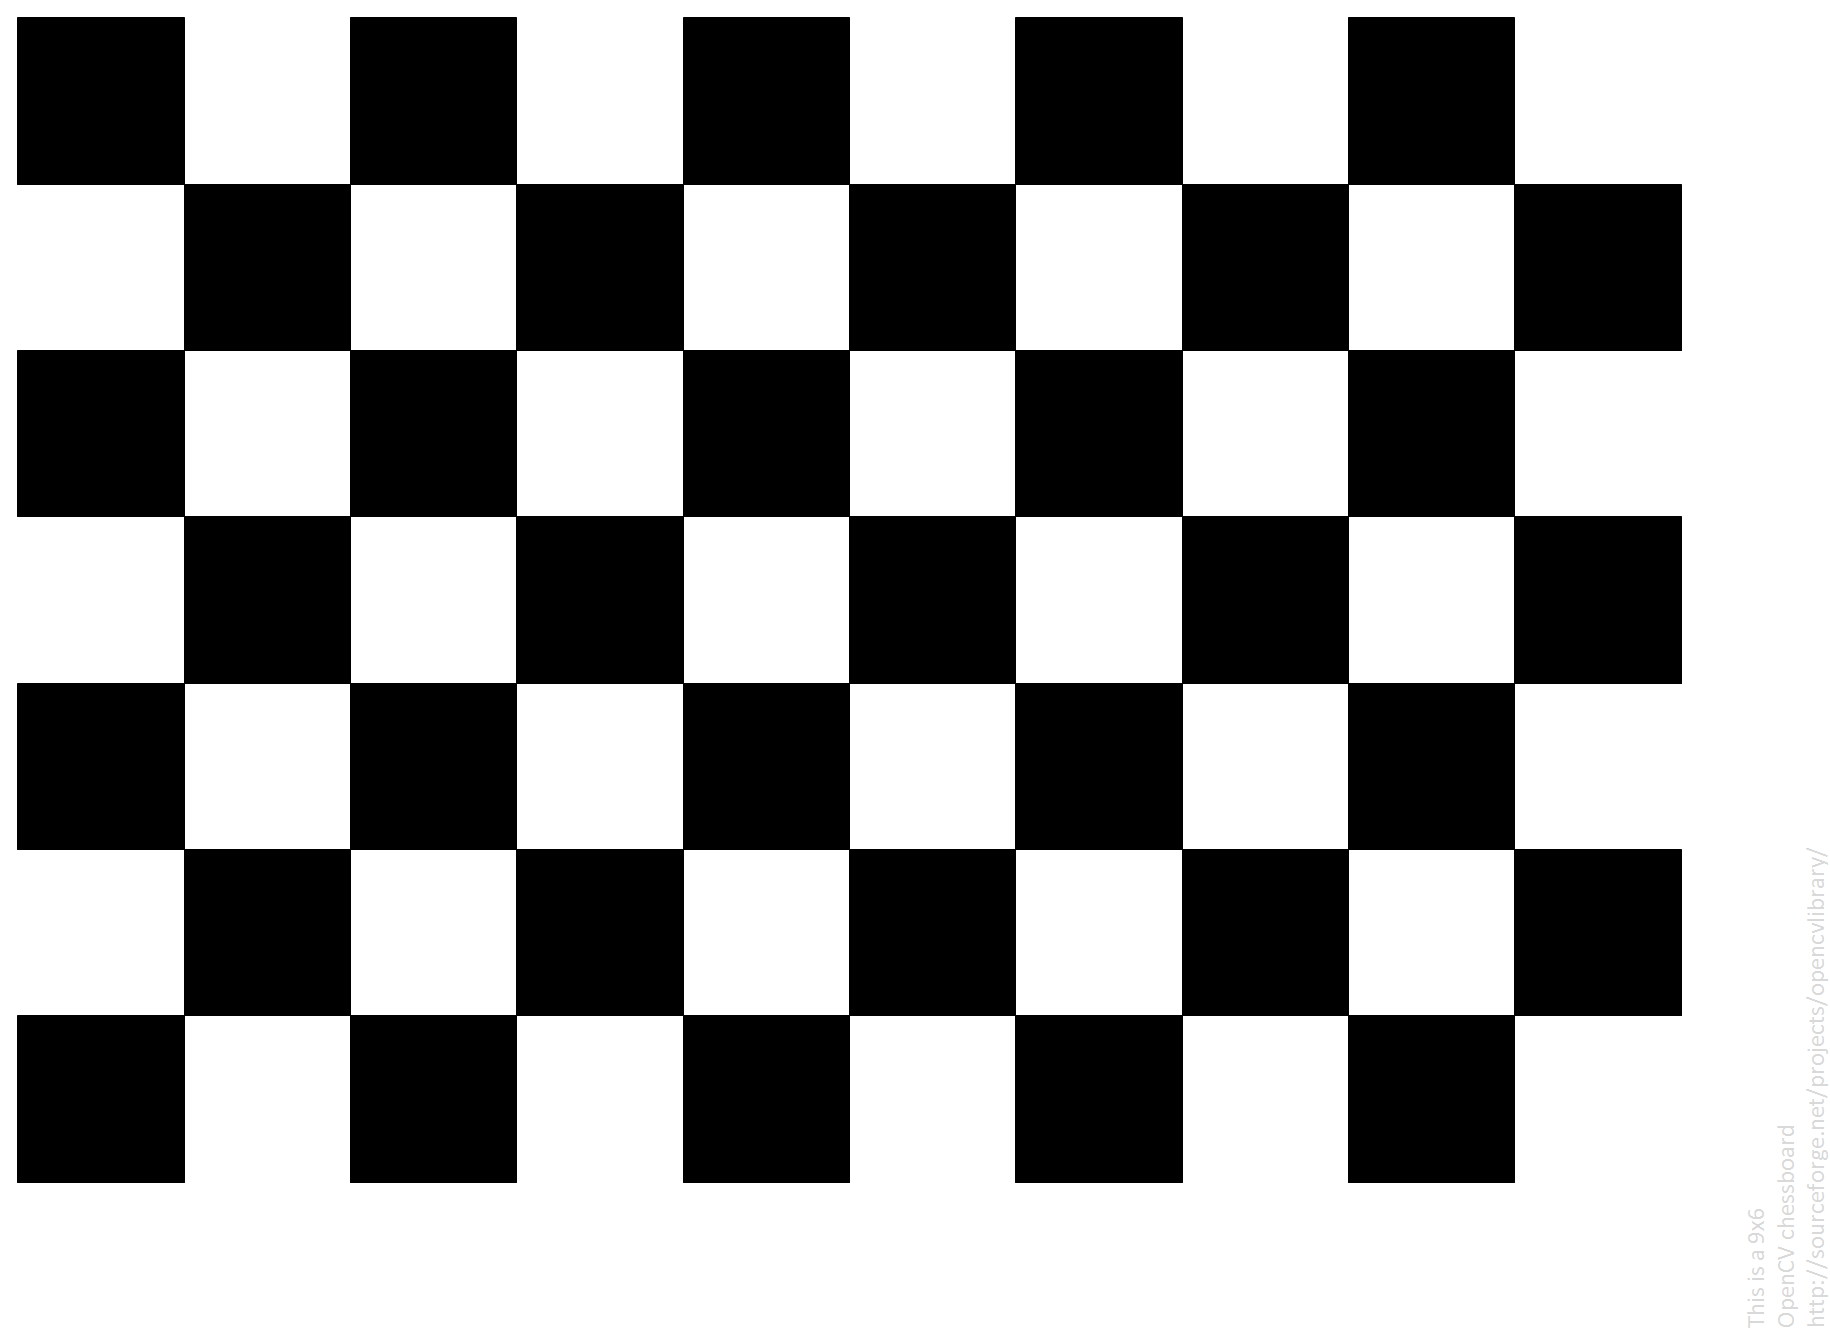
\includegraphics[width=\textwidth]{figures/checkerbord_pattern.PNG}
\caption{}
\label{fig:checkerbord_pattern}
\end{figure}


\section{From image to robot}
Once the parameters are known they need to be transformed into robot coordinates. For this the transformation matrix from the camera coordinates to robot is needed. A way to simplify this is to use a different approach than finding the camera parameters. If the camera is orthogonal to the planar space that robot needs to operate in it can be assumed that image is simply a version of the planar space with constant scaling. If a point is known in pixel coordinates and in robot coordinates it is possible to compute a simple projection between. Then it is not necessary to get the camera parameters and know the robots frame as long as the mapping is known. The mapping can be found as seen in \autoref{fig:camera_robot_shortcut} with:
\begin{equation}
\begin{split}
x_{rob}&=\theta_{0}+\theta_{1}*x_{img}+\theta_{2}*y_{img}\\
x_{rob}&=(1+*x_{img}+y_{img}) * \vec{\theta}
\end{split}
\end{equation}
 where $x_{rob}$ is the x coordinate for the robot in a place in the image space. $x_img$ and $y_img$ are the pixel coordinates of the exact same point with $\theta_1$ and $\theta_2$ is a scaling between when the robot moves in the x direction in robot coordinates how much does it move in x and y of the pixel coordinates. $\theta_0$ is the offset that comes from the robots base not having the same origin as the image. When done for both x and y the result becomes:
\begin{equation}
\begin{split}
x_{rob}&=(1+*x_{img}+y_{img})*\vec{\theta}\\
y_{rob}&=(1+*x_{img}+y_{img}) * \vec{\phi}
\end{split}
\end{equation}
where $\theta$ are the x parameters and $\phi$ is the y parameters. These can be solved for by using multiple known points and their accompanying robot and pixel coordinates like this:

\begin{equation}
\begin{bmatrix}
x_{rob1} \\
x_{rob2} \\
x_{rob3}
\end{bmatrix} 
 =
\begin{bmatrix}
1 & x_{img1} & y_{img1} & 0 \\
1 & x_{img2} & y_{img2} & 0 \\
1 & x_{img3} & y_{img3} & 0 
\end{bmatrix}  
* \vec{\theta}
\end{equation}

To then go to robot coordinates from pixel coordinates it is simply:
\begin{equation}
\begin{bmatrix}
x_{rob} \\
y_{rob} \\
\end{bmatrix} 
= 
\begin{bmatrix}
1 & x_{img} & y_{img}\\
\end{bmatrix} 
\begin{bmatrix}
\theta_0 & \phi_0 & \\
\theta_1 & \phi_1 & \\
\theta_2 & \phi_3 &  
\end{bmatrix}  
\end{equation}

\begin{figure}[h]
\centering
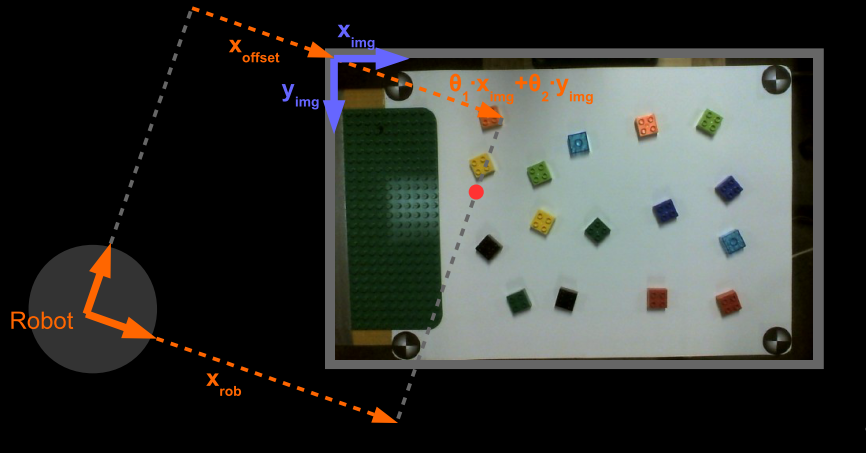
\includegraphics[width=\textwidth]{figures/camera_robot_shortcut.PNG}
\caption{}
\label{fig:camera_robot_shortcut}
\end{figure}
